\documentclass[12pt,a4paper]{article}
%
%	STARWARE - Stile base per la scrittura di documenti interni in LaTex
%

%
%	Pacchetti globali
%	Fare qui eventuali aggiunte!
%
\usepackage[utf8]{inputenc}
\usepackage[italian]{babel}
\usepackage[babel]{csquotes}
\usepackage{url}
\usepackage{graphicx}
\usepackage[colorlinks]{hyperref}
\usepackage{lastpage}
\usepackage{fancyhdr}
\usepackage[top=1cm,bottom=4cm,left=80pt,right=80pt]{geometry} %disegna la linea
\usepackage{listings} %per grandi porzioni di codice
\usepackage[table]{xcolor}
\usepackage{booktabs,tabularx}
\usepackage{makeidx}
\usepackage{fixltx2e}
\usepackage{hyperref}
\usepackage{enumitem}
\usepackage{color}
\usepackage[T1]{fontenc}
\usepackage{float}
\usepackage{svg}
\usepackage{amsmath}
\usepackage[toc]{glossaries}
\usepackage{dirtree}
\usepackage{listings}
\usepackage{siunitx}
\usepackage[official]{eurosym}
\usepackage[export]{adjustbox}
\usepackage{calc}
\usepackage{rotating}

% Per i diagrammi casi d'uso

\makeglossaries

\bibliographystyle{alpha}

%
%	VARIABILI GLOBALI
%
\newcommand{\nomeGruppo}{Basic Gym}
\newcommand{\mailGruppo}{anna.bonaldo.2@studenti.unipd.}
\newcommand{\uni}{Universit\`{a} degli Studi di Padova}
\newcommand{\uniAA}{2015/2016}

\newcommand{\prj}{Basic Gym}
\newcommand{\prjL}{Basic Gym}

\newcommand{\TF}{Thomas Fuser}
\newcommand{\LB}{Luca Boscolo}
\newcommand{\EC}{Enrico Canova}
\newcommand{\AB}{Anna Bonaldo}
\newcommand{\TFmat}{Thomas Fuser mat.1073340}
\newcommand{\LBmat}{Luca Boscolo mat.}
\newcommand{\ECmat}{Enrico Canova mat.}
\newcommand{\ABmat}{Anna Bonaldo mat.1068547}


\newcommand{\mgls}[1]{\gls{#1}\textsubscript{G}}
\newcommand{\mglspl}[1]{\glspl{#1}\textsubscript{G}}
\newcommand{\mGls}[1]{\Gls{#1}\textsubscript{G}}
\newcommand{\mGlspl}[1]{\Glspl{#1}\textsubscript{G}}



\newcommand{\latex}[1]{\texttt{#1}}
\newcommand{\fileName}[1]{\texttt{#1}}
\newcommand{\filePath}[1]{\texttt{#1}}
\newcommand{\TODO}[1]{\texttt{\large \color{red} \underline{TODO: #1}}}



%per compilare il template usare questi sotto e commentare glia altri:


\newcommand{\intestazione}[1]{

	
	
	\HRule \\[0.4cm]
	\begin{Huge}
		{\huge \bfseries #1}\\[0.4cm]
	\end{Huge}
	\HRule \\[1cm]
	\vfill
}

\newcommand{\glossarioPrint}{Al fine di evitare ogni ambiguità di linguaggio e massimizzare la comprensione dei documenti, i termini tecnici, di dominio, gli acronimi e le parole che necessitano di essere chiarite, sono riportate nel documento \GLv. Ogni occorrenza di vocaboli presenti nel \GL\ è marcata da una G maiuscola in pedice (e.g. pedice\textsubscript{G}).}

\newcommand{\descrizioneProdotto}{
Lo scopo del progetto è lo sviluppo di un sito web per la creazione e somministrazione di questionari che verranno forniti attraverso uno specifico Quiz Markup Language (\mgls{qml}). L'obiettivo è quello di creare un \mgls{software} che consenta di eseguire questionari e di visualizzare il punteggio ottenuto.I questionari disponibilili devono essere creati da docenti, i quali avranno la possibilità di scegliere le domande da inserire nel proprio questionario selezionandole tra quelle relative a vari argomenti, disponibili nel sistema.}

\newlength{\myheight}
\setlength{\myheight}{\textheight}
\addtolength{\myheight}{-2cm}

\newlength{\myheighttwo}
\setlength{\myheighttwo}{\textheight}
\addtolength{\myheighttwo}{-4cm}

\newlength{\myheightthree}
\setlength{\myheightthree}{\textheight}
\addtolength{\myheightthree}{-6cm}

\newlength{\myheightfour}
\setlength{\myheightfour}{\textheight}
\addtolength{\myheightfour}{-8cm}

%
%	Setup stili
%

\newcommand{\HRule}{\rule{\linewidth}{0.5mm}}

\definecolor{dkgreen}{rgb}{0,0.6,0}
\definecolor{gray}{rgb}{0.5,0.5,0.5}
\definecolor{mauve}{rgb}{0.58,0,0.82}
\definecolor{light}{RGB}{255,255,190}

%
%	Setup di pagina
%

%colorazione link
\hypersetup
{
	colorlinks=true,
	linkcolor=black,
	urlcolor=blue,
	citecolor=blue
}

%	Setup Header + Footer

\pagestyle{fancy}
\setlength{\headheight}{2cm} %settato grandezza header

\renewcommand{\footrulewidth}{0.5pt} %ridefinisco il valore della riga di intestazione
\renewcommand{\headrulewidth}{0.5pt} %ridefinisco il valore della riga di pie' di pagina
\addtolength{\headwidth}{\marginparsep}
\addtolength{\headwidth}{\marginparwidth}

\fancyhead{} %annulla head di default
\fancyfoot{} %annulla foot di default

%	Logo intestazione




%	footer
\cfoot{
	\uniAA\\
	\uni \\
}
\rfoot{
	\thepage\ di \pageref{LastPage}
}


% test subsubsubsection

\usepackage{titlesec}
\usepackage{hyperref}

\titleclass{\subsubsubsection}{straight}[\subsection]

\newcounter{subsubsubsection}[subsubsection]
\renewcommand\thesubsubsubsection{\thesubsubsection.\arabic{subsubsubsection}}
\renewcommand\theparagraph{\thesubsubsubsection.\arabic{paragraph}} % optional; useful if paragraphs are to be numbered

\titleformat{\subsubsubsection}
  {\normalfont\normalsize\bfseries}{\thesubsubsubsection}{1em}{}
\titlespacing*{\subsubsubsection}
{0pt}{3.25ex plus 1ex minus .2ex}{1.5ex plus .2ex}

\makeatletter
\renewcommand\paragraph{\@startsection{paragraph}{5}{\z@}%
  {3.25ex \@plus1ex \@minus.2ex}%
  {-1em}%
  {\normalfont\normalsize\bfseries}}
\renewcommand\subparagraph{\@startsection{subparagraph}{6}{\parindent}%
  {3.25ex \@plus1ex \@minus .2ex}%
  {-1em}%
  {\normalfont\normalsize\bfseries}}
\def\toclevel@subsubsubsection{4}
\def\toclevel@paragraph{5}
\def\toclevel@paragraph{6}
\def\l@subsubsubsection{\@dottedtocline{4}{7em}{4em}}
\def\l@paragraph{\@dottedtocline{5}{10em}{5em}}
\def\l@subparagraph{\@dottedtocline{6}{14em}{6em}}
\makeatother

\setcounter{secnumdepth}{4}
\setcounter{tocdepth}{4}

% A tizk picture that is resized as needed.
% It's usually instanciated with:
%       \begin{resizedtikzpicture}{\textwidth}
%           ...
%       \end{resizedtikzpicture}
\newsavebox\mybox
\newenvironment{resizedtikzpicture}[1]{%
    \def\mywidth{#1}%
    \begin{lrbox}{\mybox}%
    \begin{tikzpicture}
}{%
    \end{tikzpicture}%
    \end{lrbox}%
    \ifdim\wd\mybox>\mywidth
        \resizebox{\mywidth}{!}{\usebox\mybox}%
    \else
        \usebox\mybox %
    \fi
}


%Titolo documento
\newcommand{\titoloDocumento}{Basic Gym}

%opening
\rhead{Progetto di Tecnologie Web}
\lhead{\titoloDocumento}
\title{\titoloDocumento}


\author{Anna Bonaldo}

\begin{document}
\begin{center}
	\[  \]
	\[  \]
	\[  \]

	\vspace{1cm}
	\begin{Huge}
		\textbf{{\titoloDocumento}}\\
		\vspace{0.5cm}
	\end{Huge}
	\begin{Large}
		\textbf{Progetto di Tecnologie Web}\\
		
	\end{Large}
	\vspace{1cm}
\end{center}
 \hrule


	\begin{center}
		
		\textbf{	Informazioni sul gruppo}
		\\
		\LBmat{} \\
		\TFmat{}\\
		\ABmat{}\\
		\ECmat{}\\
		\vspace{0.5cm}
		\textbf{Informazioni sul sito }\\
		\url{http://tecnologie-web.studenti.math.unipd.it/tecweb/~tfuser}
	\end{center}
	\vspace{0.5cm}
		\hrule	
	\begin{center}
		\textbf{Credenziali accesso amministratore}\\
		\textit{username} \texttt{admin}\\
		\textit{pw} \texttt{admin}\\
		\vspace{0.5cm}
		\textbf{Credenziali accesso utente 1}\\
		\textit{username} \texttt{annabonaldo@gmail.com}\\
		\textit{pw} \texttt{ciaociaociao}\\
		\vspace{0.5cm}
		\textbf{Credenziali accesso utente 2}\\
		\textit{username} \texttt{thomasfuser@gmail.com}\\
		\textit{pw} \texttt{ciaociaociao}\\
	\end{center}


	\newpage
	\tableofcontents
	
	\newpage
\section{Utenza del sito}
\subsection{Raggiungere l'informazione in un numero minimo di click}
\subsubsection{Utente non registrato}
\paragraph{Minimo numero di click}Un utente non registrato che accede al sito accede con un solo click dal menu a tutte le infomrmazioni principali maggiormente significative.
Le pagine di dettaglio, dedicate agli utenti che necessitano di approfondire le informazioni e più motivati sono quelle raggiungibili in due click. 
\paragraph{Tipologia dell'utenza}Non è possibile fare particolari assunzioni sull'utenza di un sito di questo tipo, ne' sugli strumenti utilizzati per accedervi. Si è cercato pertanto di massimizzarne il supporto da parte dei browser e l'accessibilità.
\subsubsection{Utente registrato} Per l'utente registrato mantiene lo stesso schema del sito dell'utente non registrato. In questo modo l'utente conosce già la struttura deli sito. Un utente registrato è in grado di acquistare gli abbonamenti offerti dalla palestra.
Vengono aggiunte alcune funzionalità al menù e alla pagina prezzi e la pagina di riepilogo degli abbonamenti acquistati e delle informazioni di profilo.
\subsubsection{Amministratore} L'amministratore ha la possibilità di gestire gli abbonamenti offerti dalla palestra. E' in grado di modificare, aggiungere o rimuovere un abbonamento. 
\paragraph{Tipologia di utente amministratore}Si assume che l'amministratore non sia interessato a danneggiare il proprio sito e che si tratti di un'utente esperto. Nonostante ciò i maggiori provvedimenti per la sicurezza sono stati aggiunti anche alle pagine amministratore.
\paragraph{Sito completo} Per l'amministratore si è mantenuta la possibilità di visualizzare tutte le pagine del sito una volta effettuato l'accesso, per garantire il minor numero di ostacoli alla navigazione, come la necessità di "uscire" dal profilo amministratore per visualizzare alcune pagine.

\section{Presentazione}
\subsection{Schema dei colori}
\paragraph{Colori safe}
I colori utilizzati nel sito sono esclusivamente colori safe. In particolare sono stati usati
\begin{center}
	\textbf{Colori Safe utilizzati}
	
	\begin{tabular}{c c c c c}
		\midrule  \#000 & \#333 & \#CCC & \#EEE  &  \#FFF \\ \midrule 
	\end{tabular} 
\end{center}
\subsubsection{Contrasto}
\paragraph{Colore dei link}
\begin{itemize}
	\item \textit{\textbf{Link non visitati}} \#FFCC33 è stato utilizzato per i link per massimizzare il contrasto con \#000, \#333 ed essere distinguibile dal colore dei link visitati. Inoltre per adeguarsi alle convenzioni i link utilizzano \textbf{testo sottolineato.}
	\item \textbf{\textit{Link visitati} :\#FFF }è stato utilizzato per i link visitati. Questi mantengono il testo sottolineato cambiando solamente colore da \#FFCC33 a \#FFF. 
\end{itemize}

\subsection{Test  }
\subsubsection{Color blindness test}
Per l'accessibilità relativa al daltonismo o alla difficoltà di visualizzare i colori è stato usato lo strumento online: 	
\begin{center}
	\url{http://www.color-blindness.com/coblis-color-blindness-simulator/}
\end{center}
Si riporta solamente la versione del sito visualizzato in modalità monocromatica, in quanto rappresenta la situazione peggiore. 
In ogni caso, grazie ai colori scelti, l'accessibilità risulta ottima. 
\begin{figure}[h]
\centering
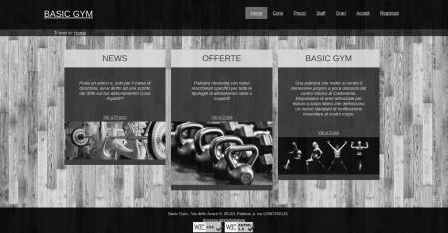
\includegraphics[width=0.6\linewidth]{img/colorblind/07}
\caption{Visione monocromatica del sito}
\label{fig:07}
\end{figure}


\subsection{Test del contrasto}
Il contrasto tra testo e sfondo è stato verificato attraverso il sito 
\begin{center}
	\url{http://webaim.org/resources/contrastchecker/}
\end{center}
ottenendo un una \textbf{valutazione WCAG AAA} per tutte le combinazioni utilizzate per sia \textbf{testo di grandezza normale che grande.}

\subsection{Accessibilità della presentazione}
\paragraph{Dimensioni e unità di misura} La dimensione del testo viene specificata in \textbf{em} e le dimensioni degli elementi della pagina vengono specificate in percentuale qual ora debbano dipendere dalla dimensione dello schermo e in em quando devono dipendere dalla dimensione del font preferito dall'utente. 

\subsection{Presentazione per dispositivi Mobile}
La presentazione del sito viene adattata alla dimensione dello schermo del dispositivo utilizzato per accedervi. 
Per schermi di dimensioni ridotte la presentazione viene riadattata in modo da sfruttare al meglio lo spazio disponibile e rendere accessibili i contenuti. 
\paragraph{Tabella orario}
L'orario viene presentato sotto forma di tabella. Accedendo al sito da mobile il contenuto viene presentato in modo da renderlo accessibile anche da un piccolo schermo. 
Il contenuto della pagina e il codice Html non viene modificato e resta accessibile, preservando la completa separazione tra presentazione e contenuto. 

\paragraph{Spazio ai contenuti} Per tutte le pagine del sito, nella versione mobile viene ridotto lo spazio destinato alle immagini e in caso di schermi particolarmente ridotti queste vengono nascoste, lasciando spazio al testo e al contenuto, prioritari per l'utente. 
I margini vengono eliminati e tutto lo spazio disponibile viene utilizzato per i contenuti delle pagine.

\paragraph{Menu mobile} Il menu nella versione mobile del sito viene trasformato in un tasto che utilizza l'icona classica, utilizzata anche dai browser per indicare il menu. 
Il codice html della pagina non viene modificato, si tratta solamente della presentazione. 
Il menu mobile viene posizionato in alto a destra, la posizione considerata più accessibile da dispositivi mobile. 
Per motori di ricerca particolarmente obsoleti, che non supportano particolari funzionalità CSS il menu resta comunque visibile come nella modalità desktop.
\subsection{CSS3 e retrocompatibilità}
Il CSS3 offre numerose possibilità per un web designer attento all'estetica della propria pagina. 
Si è deciso pertanto di non limitarsi al CSS2, ma le scelte adottate massimizzano non solo la retrocompatibilità del sito e dei contenuti ma anche dell'aspetto grafico. 
Le regole CSS3 vengono utilizzate per dare un'aspetto maggiormente curato nei dettagli al sito che risulta esteticamente gradevole in ogni caso. 
Tali regole vengono sempre posizionate a fine blocco per non impedire che l'interpretazone delle altre regole del blocco sia compromessa. 
\section{Contenuto}
\subsection{XHTML Strict}
Poichè non era possibile fare assunzioni sui mezzi utilizzati dall'utenza si è utilizzato HTML Strict per massimizzare la retrocompatibilità. 
\subsection{Separazione da presentazione e comportamento}
\subsection{Utilizzo corretto dei tag}
Il contenuto è completamente separato dalla presentazione e dal comportamento. 
Si è creato in prima istanza solo il contenuto come codice XHtml. Il codice css è stato aggiunto in un momento successivo, allegando un file apposito tramite i tag meta. 
Il riferimento al contenuto viene effettuato solamente tramite appositi id, classi e elementi del codice html. 
 
\subsection{Le immagini}
Le immagini vengono inserite nel codice html solamente se \textbf{utili al contenuto} della pagina. 
Qualora costituiscano un abbellimento della presentazione del sito vengono inserite da CSS. 
Tutte le immagini utili al contenuto prenti nel codice html presentano un \textbf{attributo "alt"} che ne esplicita il contenuto a screen reader e motori di ricerca. 

\subsubsection{La lingua} La lingua utilizzata nel sito è specificata nei tag meta per il contenuto in generale. 
Le parole in altre lingue presenti nel testo sono contrassegnate dall'\textbf{attributo "xml:lang"}  e inserite in un'apposito \textbf{tag span}.

\section{Accessibilità e form}
\subsection{Errori nell'inserimento dei dati}
La gestione degli errori nei form avviene su due livelli:
\begin{itemize}
	\item \textbf{Controlli lato client: javascript} effettuato \textit{on-bleur} per evitare all'utente di dover inviare il form per accorgersi degli errori.
	\item \textbf{Controlli lato server: perl} tutti i controlli vengono effettuati anche lato server, in modo da garantire l'integrità del database, l'accessibilità e controlli sull'inserimento di script nocivi anche se l'utente disabilita javascript.
\end{itemize}
\subsubsection{Segnalazione di errori nei dati inseriti}
\paragraph{Posizione} Le segnalazioni degli errori relativamente a inserimento di dati scorretti viene visualizzato in un \textbf{tag span} posizionato il più vicino possibile alla casella di inserimento dei dati che ha scatenato l'errore. Questo per aumentare l'accessibilità e diminuire il sovraccarico congnitivo. 
\paragraph{Segnalazione di errori "precise" e utili alla correzione} Per l'utente deve essere chiaro il motivo per cui l'inserimento del dato ha scatenato un errore. Pertanto si cerca di specificare chiaramente e in modo preciso perchè l'inserimento non è corretto e risulta semplice correggere l'errore: si aumenta così l'accessibilità e diminuire il sovraccarico cognitivo. 
\paragraph{Convenzioni interne per la presentazione degli errori} Per rendere evidenti gli errori rispetto al resto del testo e degli elementi della pagina viene utilizzata una presentazione apposita per questi ultimi omogenea per tutti i form del sito, in modo da non rompere le convenzioni interne.
\paragraph{Mantenimento dei dati inseriti in caso di errore} 
Nel caso in cui un campo dati scateni un'errore l'utente non è costretto a reinserire tutti i dati ma è sufficiente che corregga l'inserimento precedente in corrispondenza dell'errore. 
\subsection{Form di grandi dimensioni: la registrazione} 
La \textbf{registrazione} richiede l'inserimento di un notevole numero di dati. Per questo motivo il form è stato spezzato in una successione di form per non scoraggiare l'utente e rendere più semplice la segnalazione dei dati e rendere più piacevole l'esperienza all'utente. 
\paragraph{Passaggio dei parametri} Per il passaggio dei parametri vengono utilizzati i \textbf{campi hidden}. 
\paragraph{Quanto manca?} L'utente deve sapere a che punto si trova nel processo di registazione. Per questo viene indicato in alto, a fianco del titolo del form quanti form restano da compilare
\section{Gestione e salvataggio dei dati}
\subsection{Lo schema dei dati}
Lo schema per i dati è stato modellato secondo il \textbf{modello "tende alla veneziana"} per consentire maggiore flessibilità e la possibilità di dichiarare più di un elemento radice.
In questo modo un unico schema riusciva a raccogliere tutti i tipi necessari a modellare i dati.

\paragraph{XmlSchema e date} Per i tipi "data" si è scelto di utilizzare il \textbf{tipo predefinito} fornito dall'\textbf{XmlSchema}. In questo modo era possibile avere un controllo sul contenuto dello schema. Le date vengono pertanto trasformate in un apposito formato in lettura e scrittura attraverso il linguaggio Perl. 
\subsection{Il database: le istanze dello schema}
Per il salvataggio dei dati si è preferito mantenere separati i dati relativi agli utenti, agli amministratori e agli abbonamenti della palestra. 
Questa scelta è stata necessaria per mantenare flessibili le funzinalità offerte dal sito e aumentarne la manutenibilità.
La coerenza tra il contenuto delle varie parti del database è garantita dalla definizione di un'unico schema. 
\subsection{Validazione delle pagine}
Le pagine in codice html sono state validate attraverso il validatore disponibile ne sito \url{https://validator.w3.org/}. Anche il codice css è stato validato attraverso questo servizio online. 
Gli schemi XML e le relative istanze sono state validate attraverso strumenti online e strumenti forniti dall'editor Notepad++. 
\appendix
\section{Struttura del sito}
\subsection{cgi-bin}
\begin{itemize}
	\item \texttt{index.cgi}
	\item \texttt{form\_reg1.cgi} gestione dei controlli del primo form di registrazione. 
	\item \texttt{form\_reg2.cgi} gestione dei controlli del secondo form di registrazione.
	\item \texttt{form\_reg3.cgi} gestione dei controlli del terzo form di registrazione.
	\item \texttt{form\_reg4.cgi} gestione dei controlli del quarto form di registrazione e inserimento dei dati utente nel database.
	\item \texttt{corsi.cgi} pagina di paroramica dei corsi.
	\item \texttt{cardio.cgi} pagina di descrizione corsi cardio-fitness.
	\item \texttt{soft.cgi}pagina di descrizione corsi soft-fitness.
	\item \texttt{orario.cgi} orario dei corsi. 
	\item \texttt{prezzi.cgi} prezzi (utente non loggato, utente loggato e amministratore).
	\item \texttt{login.cgi} gestione login. 
	\item \texttt{login\_admin.cgi}gestione login amministratore.
	\item \texttt{logout.cgi} gestione logout.
	\item \texttt{utente.cgi}	pagina di riepilogo profilo utente e abbonamenti acquistati. 
	\item \texttt{riepilogoAggiunta.cgi} gestione del riepilogo di aggiunta di un abbonamento (amministratore).
	\item \texttt{reipilogoModificaAbbonamento.cgi} gestione del riepilogo di modifica di un abbonamento (amministratore).
	\item \texttt{registrazione.cgi}  pagina di registrazione.
	\item\textbf{ \texttt{util}}
	\subitem \texttt{html\_util.pm} stampa di header e meta tag, footer, menu di primo e secondo livello, breadcrumb. 
	\subitem \texttt{html\_content.pm} funzioni di stampa dei contenuti html delle pagine utente.
	\subitem \texttt{html\_content\_admin.pm}  di stampa dei contenuti html delle pagine amministratore. 
	\subitem \texttt{base\_util.pm} stampa dei form di registrazione. 
	\subitem \texttt{db\_util.pm} funzioni di utilità di lettura e scrittura del database. 
\end{itemize}

\subsection{public\_html}
\begin{itemize}
	\item \texttt{index.html } pagina che effettua il redirect alla pagina \texttt{index.cgi}.
	\item \texttt{\textbf{css}}
		\subitem \texttt{style.css} css versione desktop e mobile. 
		\subitem \texttt{print.css} css per la stampa.
	\item\texttt{\textbf{ js}}
	\subitem \texttt{registrationLong.js} controlli lato client. 
\end{itemize}
\subsection{data}
\begin{itemize}
	\item \texttt{schema.xsd} schema dei dati. 
	\item \texttt{utente.xml} database dei dati degli utenti registrati. 
	\item \texttt{prezzi.xml} database degli abbonamenti offerti dalla palestra. 
	\item \texttt{admin.xml} dati amministratore. 
\end{itemize}

\section{Organizzazione del gruppo}
\paragraph{\TF{}}
\begin{itemize}
	\item \textbf{HTML}
	\subitem pagina staff
	\item \textbf{CSS}
	\subitem pagina staff
	\item\textbf{Perl}
	\subitem pagina utente (abbonamenti utente)
	\subitem pagina prezzi e gestione prezzi lato amministratore
	\item \textbf{Javascript}
	\subitem Controlli form lato client
	\item Validazione
	\subitem validazione html
	\subitem validazione css
	
	
\end{itemize}
\paragraph{\LB{}}
\begin{itemize}
	\item \textbf{Html}
	\subitem hompage
	\subitem pagine di login utente e amministratore
	\item\textbf{CSS}
	\subitem homepage
	\subitem menu di primo livello (desktop e mobile)
	\subitem breadcrump
	\subitem footer
	\item \textbf{Perl}
	\subitem pagina prezzi lato amministratore;
	\subitem controllo di sessione;
	\subitem login e logout;
\end{itemize}
\paragraph{\AB{}}
\begin{itemize}
	\item \textbf{Html}
	\subitem registrazione
	\subitem pagina orario versione desktop
	\subitem utente
	\subitem corsi, pagine di dettaglio dei corsi
	\item \textbf{CSS}
	\subitem orario
	\subitem pagine corsi e pagine di dettaglio dei corsi
	\subitem pagina profilo utente
	\subitem form, login e registrazione
	\item \textbf{Perl}
	\subitem Registrazione
	\subitem Pagina utente(profilo utente)
	\subitem Controlli su input form lato server (inserimento prezzi,modifica prezzi, registrazione )
	\item\textbf{XML}
	\subitem schemi xml (utenti.xsd, prezzi.xsd )

\end{itemize}
\paragraph{\EC{}}
\begin{itemize}
	\item\textbf{CSS}
	\subitem pagina orario versione mobile
	\item\textbf{Javascript}
	\subitem Controlli form lato client
	\item\textbf{ Perl}
	\subitem parte pagina utente
\end{itemize}

\end{document}
